% =============================================================================
% StructureTower 数論シリーズ NT1: 分岐塔
% LuaLaTeX document — Lean 4 形式化の数学的解説
% =============================================================================
\documentclass[a4paper,11pt]{ltjsarticle}

% --- Core packages ---
\usepackage{luatexja-fontspec}
\usepackage{amsmath,amssymb,amsthm}
\usepackage{mathtools}
\usepackage{tikz}
\usepackage{tikz-cd}
\usetikzlibrary{cd,arrows,decorations.pathmorphing,matrix,positioning,shapes,calc}
\usepackage{enumitem}
\usepackage{hyperref}
\usepackage{cleveref}
\usepackage{tcolorbox}
\usepackage{listings}
\usepackage{xcolor}
\usepackage{geometry}
\usepackage{fancyhdr}
\usepackage{float}
\usepackage{booktabs}
\usepackage{array}

% --- Page geometry ---
\geometry{margin=2.5cm, top=3cm, bottom=3cm}

% --- Fonts ---
\setmainjfont{Noto Serif JP}
\setsansjfont{Noto Sans JP}

% --- Colors ---
\definecolor{leanblue}{HTML}{2563EB}
\definecolor{leanbg}{HTML}{F8FAFC}
\definecolor{leancomment}{HTML}{6B7280}
\definecolor{leankeyword}{HTML}{7C3AED}
\definecolor{leanstring}{HTML}{059669}
\definecolor{accentcolor}{HTML}{1E40AF}
\definecolor{theoremcolor}{HTML}{EFF6FF}
\definecolor{definitioncolor}{HTML}{F0FDF4}
\definecolor{remarkcolor}{HTML}{FFF7ED}

% --- Hyperref ---
\hypersetup{
  colorlinks=true,
  linkcolor=accentcolor,
  urlcolor=leanblue,
  citecolor=accentcolor,
  pdftitle={StructureTower 数論シリーズ NT1: 分岐塔},
  pdfauthor={su},
}

% --- Theorem environments ---
\theoremstyle{definition}
\newtheorem{definition}{定義}[section]
\newtheorem{example}[definition]{例}

\theoremstyle{plain}
\newtheorem{theorem}[definition]{定理}
\newtheorem{lemma}[definition]{補題}
\newtheorem{proposition}[definition]{命題}
\newtheorem{corollary}[definition]{系}

\theoremstyle{remark}
\newtheorem{remark}[definition]{注意}

% --- Lean code environment ---
\lstdefinelanguage{lean4}{
  morekeywords={def,theorem,lemma,example,instance,class,structure,
    where,let,in,do,if,then,else,match,with,fun,return,
    import,open,namespace,section,end,variable,
    inductive,abbrev,noncomputable,private,protected,
    sorry,admit,have,show,suffices,calc,by,exact,
    apply,intro,intros,constructor,cases,induction,
    simp,rw,rfl,ext,ring,linarith,omega,norm_num,
    decide,trivial,assumption,contradiction,
    Type,Prop,Sort,Set,true,false,
    attribute,deriving},
  sensitive=true,
  morecomment=[l]{--},
  morecomment=[n]{/-}{-/},
  morestring=[b]",
}

\lstnewenvironment{leancode}[1][]{%
  \lstset{
    language=lean4,
    basicstyle=\ttfamily\small,
    keywordstyle=\color{leankeyword}\bfseries,
    commentstyle=\color{leancomment}\itshape,
    stringstyle=\color{leanstring},
    backgroundcolor=\color{leanbg},
    frame=single,
    rulecolor=\color{leanblue!30},
    framesep=8pt,
    xleftmargin=12pt,
    xrightmargin=12pt,
    breaklines=true,
    breakatwhitespace=true,
    showstringspaces=false,
    tabsize=2,
    captionpos=b,
    numbers=left,
    numberstyle=\tiny\color{leancomment},
    numbersep=8pt,
    aboveskip=1em,
    belowskip=1em,
    inputencoding=utf8,
    extendedchars=true,
    literate=
      {->}{{\(\to\)}}1
      {<->}{{\(\leftrightarrow\)}}1
      {<=}{{\(\leq\)}}1
      {>=}{{\(\geq\)}}1
      {/=}{{\(\neq\)}}1
      {:=}{{:=}}2,
    #1
  }%
}{}

% --- Tcolorbox styles ---
\tcbuselibrary{skins,breakable}

\newtcolorbox{proofstrategy}{
  colback=remarkcolor,
  colframe=orange!60!black,
  title={\textbf{証明戦略}},
  fonttitle=\sffamily,
  boxrule=0.5pt,
  arc=3pt,
}

\newtcolorbox{mathinsight}{
  colback=theoremcolor,
  colframe=accentcolor,
  title={\textbf{数学的洞察}},
  fonttitle=\sffamily,
  boxrule=0.5pt,
  arc=3pt,
}

\newtcolorbox{parallelbox}{
  colback=definitioncolor,
  colframe=green!50!black,
  title={\textbf{環と群の並行性}},
  fonttitle=\sffamily,
  boxrule=0.5pt,
  arc=3pt,
}

% --- Math macros ---
\newcommand{\ST}{\mathsf{ST}}
\newcommand{\Hom}{\mathrm{Hom}}
\newcommand{\id}{\mathrm{id}}
\newcommand{\op}{\mathrm{op}}
\newcommand{\Nat}{\mathbb{N}}
\newcommand{\ZZ}{\mathbb{Z}}
\newcommand{\Gal}{\mathrm{Gal}}
\newcommand{\Aut}{\mathrm{Aut}}
\newcommand{\ord}{\mathbb{N}^{\mathrm{op}}}
\newcommand{\iInf}{\displaystyle\bigcap}
\newcommand{\sgcl}{\mathrm{sgClosure}}
\newcommand{\rambreak}{b(\sigma)}

% --- Header/Footer ---
\pagestyle{fancy}
\fancyhf{}
\renewcommand{\headrulewidth}{0.4pt}
\fancyhead[L]{\small\sffamily\nouppercase{\leftmark}}
\fancyhead[R]{\small\sffamily Lean 4 形式化 --- NT1}
\fancyfoot[C]{\thepage}

% =============================================================================
\begin{document}

% --- Title ---
\title{%
  {\LARGE\sffamily\bfseries StructureTower 数論シリーズ NT1}\\[0.5em]
  {\large\sffamily 分岐塔：群のフィルトレーションと数論的構造}\\[0.3em]
  {\normalsize\sffamily Lean 4 / Mathlib4 による形式化とその数学的解説}%
}
\author{su}
\date{\today}
\maketitle
\thispagestyle{fancy}

% --- AI Disclosure ---
\begin{center}
\small
\textit{AI assistance disclosure:}\\
Lean ソースコードは Claude (Anthropic) で骨格を生成し、
Codex (OpenAI) で修正した。\\
\TeX\ 文書は Claude Code (Anthropic) で生成した。\\
著者による加筆・修正は行っていない。\\
内容の正確性は保証されず、誤りがあれば著者の責任である。
\end{center}

\vspace{1em}

% --- Abstract ---
\begin{abstract}
本稿は Lean 4 / Mathlib4 による形式化ファイル
\texttt{StructureTower\_NT1\_RamificationTower.lean} の数学的解説である。
\textsc{StructureTower} フレームワークを用いて，群のフィルトレーション，
特に局所体のガロア拡大における\textbf{分岐フィルトレーション}を形式化する。
$G = G_0 \supseteq G_1 \supseteq G_2 \supseteq \cdots$ という
正規部分群の減少列を $\textsc{StructureTower}\,\mathbb{N}^{\mathrm{op}}\,G$ として捉え，
L5 で構築した \texttt{idealPowTower}（環のイデアル冪塔）との完全な並行性を証明する。
主要な結果として，部分群フィルトレーション塔の構成（§1），
正規鎖・閉包性・共役自己射（§2），
分岐塔の公理的定義と交換子条件（§3），
分離条件と脱出定理（§4），
環と群の二重フィルトレーションを結ぶ橋（§5）を解説する。
\end{abstract}

\tableofcontents
\newpage

% =============================================================================
\section{はじめに：動機と全体像}
% =============================================================================

\subsection{数論への動機}

L5--L7 では可換環 $R$ 上のイデアル $I$ の冪による\textbf{$I$-進フィルトレーション}
\[
  R \supseteq I \supseteq I^2 \supseteq I^3 \supseteq \cdots
\]
を \textsc{StructureTower} の言語で形式化した。
これは環論の「加法側」の構造である。

本稿の数論シリーズ NT1 では，その\textbf{群側の対応物}を構築する。
動機は\textbf{局所体のガロア拡大における分岐フィルトレーション}である。
局所体の拡大 $L/K$，ガロア群 $G = \Gal(L/K)$，
$L$ の均一化元 $\pi$，付値 $v_L$ に対し，
\[
  G_i = \{\,\sigma \in G \mid v_L(\sigma(\pi) - \pi) \geq i + 1\,\}
  \quad (i \geq 0)
\]
として定義される正規部分群の列
\[
  G = G_{-1} \supseteq G_0 \text{（惰性群）} \supseteq G_1 \text{（暴分岐群）}
  \supseteq G_2 \supseteq \cdots
\]
が分岐フィルトレーションである（図~\ref{fig:ramification-tower}）。

\begin{figure}[H]
\centering
\begin{tikzpicture}[node distance=1.8cm,>=stealth]
  \node (G) {$G = G_{-1}$};
  \node (G0) [below of=G] {$G_0$（惰性群）};
  \node (G1) [below of=G0] {$G_1$（暴分岐群）};
  \node (G2) [below of=G1] {$G_2$};
  \node (dots) [below of=G2] {$\vdots$};
  \node (triv) [below of=dots] {$\{1\}$};
  \draw[right hook->] (G0) -- (G) node[midway,right] {\small $\trianglelefteq$};
  \draw[right hook->] (G1) -- (G0) node[midway,right] {\small $\trianglelefteq$};
  \draw[right hook->] (G2) -- (G1) node[midway,right] {\small $\trianglelefteq$};
  \draw[right hook->] (dots) -- (G2);
  \draw[right hook->] (triv) -- (dots);
  \node[right=3cm of G0, text width=4.5cm] (ann0)
    {\small $G_0/G_1 \cong \mathbb{F}_q^\times$（巡回群）};
  \node[right=3cm of G1, text width=4.5cm] (ann1)
    {\small $G_1/G_2$ は $p$-群（$p = \mathrm{char}\,\mathbb{F}_q$）};
  \node[right=3cm of G2, text width=4.5cm] (ann2)
    {\small $G_i/G_{i+1}$ は $\mathbb{F}_q$-加法群};
  \draw[dashed,->] (G0) -- (ann0);
  \draw[dashed,->] (G1) -- (ann1);
  \draw[dashed,->] (G2) -- (ann2);
\end{tikzpicture}
\caption{局所体 $L/K$ の分岐フィルトレーション。各 $G_i$ は $G$ の正規部分群。
商群の構造が分岐の深さを反映する。}
\label{fig:ramification-tower}
\end{figure}

\subsection{idealPowTower との並行性}

本稿の核心的観察は，環の $I$-進フィルトレーションと群の分岐フィルトレーションが
\textsc{StructureTower} の枠組みで完全に並行に記述できるという点である（表~\ref{tab:parallel}）。

\begin{table}[H]
\centering
\caption{環（L5）と群（NT1）の対比}
\label{tab:parallel}
\renewcommand{\arraystretch}{1.3}
\begin{tabular}{lll}
\toprule
\textbf{概念} & \textbf{L5（環）} & \textbf{NT1（群）} \\
\midrule
基本構造 & \texttt{idealPowTower} $I$ & \texttt{subgroupFiltrationTower} $f$ \\
添字集合 & $\mathbb{N}^{\mathrm{op}}$ & $\mathbb{N}^{\mathrm{op}}$ \\
零/単位元の帰属 & $0 \in I^n$（$\forall n$） & $1 \in G_n$（$\forall n$） \\
閉性 & $I^n$ はイデアル & $G_n$ は部分群 \\
ClosedTower & \texttt{idealClosure} & \texttt{subgroupClosure} \\
乗法互換性 & $I^m \cdot I^n \subseteq I^{m+n}$ & $[G_i,G_j] \leq G_{i+j}$ \\
分離条件 & $\bigcap_n I^n = \bot$ & $\bigcap_n G_n = \bot$ \\
脱出定理 & $x \neq 0 \Rightarrow \exists n,\,x \notin I^n$ & $\sigma \neq 1 \Rightarrow \exists n,\,\sigma \notin G_n$ \\
非自明な射 & 環準同型 $\to$ \texttt{Hom} & 共役写像 $\to$ \texttt{Hom} \\
\bottomrule
\end{tabular}
\end{table}

\subsection{Lean 4 形式化のインポート}

\begin{leancode}
import Mathlib.Data.Set.Lattice
import Mathlib.Order.GaloisConnection.Basic
import Mathlib.Order.Closure
import Mathlib.Algebra.Group.Subgroup.Basic
import Mathlib.Algebra.Group.Subgroup.Lattice
import Mathlib.GroupTheory.Index
import Mathlib.GroupTheory.Coset.Basic
import Mathlib.RingTheory.Ideal.Operations
import Mathlib.Data.Nat.Find
\end{leancode}

% =============================================================================
\section{§NT1-1. 部分群フィルトレーション塔}
% =============================================================================

\subsection{設計方針}

\textbf{入力}: 反単調な部分群列
$f\colon \mathbb{N} \to \mathrm{Subgroup}\,G$，
すなわち $i \leq j \Rightarrow f(j) \leq f(i)$。

\textbf{設計判断}: \textsc{StructureTower} は増加族を要求するため，
順序双対 $\mathbb{N}^{\mathrm{op}}$ で添字付けする。
$\mathrm{level}(n) := \lvert f(\mathrm{ofDual}(n))\rvert$
（部分群の台集合）とすることで，L5 の \texttt{idealPowTower} と完全に並行になる。

\begin{figure}[H]
\centering
\begin{tikzcd}[column sep=3cm]
  \mathbb{N}
    \arrow[r, "f", "{\text{反単調}}"']
  & (\mathrm{Subgroup}\,G)^{\mathrm{op}} \\
  \mathbb{N}^{\mathrm{op}}
    \arrow[u, "\mathrm{ofDual}"]
    \arrow[r, dashrightarrow, "\text{level}"']
  & \mathcal{P}(G)
    \arrow[u, "\text{台集合}"']
\end{tikzcd}
\caption{\texttt{subgroupFiltrationTower} の構成。
$\mathbb{N}^{\mathrm{op}}$ から $\mathcal{P}(G)$ への単調写像を，
反単調な部分群列 $f$ から誘導する。}
\label{fig:subgroup-tower-construction}
\end{figure}

\begin{definition}[部分群フィルトレーション塔]\label{def:subgroup-filtration-tower}
  群 $G$ と反単調写像 $f\colon \mathbb{N} \to \mathrm{Subgroup}\,G$
  （順序射 $f\colon \mathbb{N} \to (\mathrm{Subgroup}\,G)^{\mathrm{op}}$ と等価）
  に対し，
  \[
    \texttt{subgroupFiltrationTower}(f)
    \;:=\;
    \bigl(\mathrm{level}(n) = \lvert\mathrm{ofDual}(f(\mathrm{ofDual}(n)))\rvert\bigr)_{n \in \mathbb{N}^{\mathrm{op}}}
  \]
  は $\textsc{StructureTower}\,\mathbb{N}^{\mathrm{op}}\,G$ を定める。
\end{definition}

\begin{proofstrategy}
単調性の確認：$i \leq j$ in $\mathbb{N}^{\mathrm{op}}$
$\Leftrightarrow$ $\mathrm{ofDual}(j) \leq \mathrm{ofDual}(i)$ in $\mathbb{N}$
$\Rightarrow$ $f(\mathrm{ofDual}(i)) \leq f(\mathrm{ofDual}(j))$ in $(\mathrm{Subgroup}\,G)^{\mathrm{op}}$
（$f$ が $\mathbb{N} \to (\mathrm{Subgroup}\,G)^{\mathrm{op}}$ の順序射であることから）
$\Rightarrow$ $\lvert f(\mathrm{ofDual}(i))\rvert \subseteq \lvert f(\mathrm{ofDual}(j))\rvert$。
\end{proofstrategy}

\begin{leancode}
def subgroupFiltrationTower (f : N ->o (Subgroup G)^od) :
    StructureTower N^od G where
  level n := (OrderDual.ofDual (f (OrderDual.ofDual n)))
  monotone_level := by
    intro i j hij x hx
    have h := f.monotone (OrderDual.ofDual_le_ofDual.mpr hij)
    exact h hx
\end{leancode}

\subsection{基本性質}

\begin{proposition}[単位元の帰属]\label{prop:one-mem}
  すべてのレベル $n \in \mathbb{N}^{\mathrm{op}}$ に対し，$1 \in \mathrm{level}(n)$。
\end{proposition}

\begin{proof}
  $\mathrm{level}(n) = \lvert H_n \rvert$（$H_n$ は部分群）であり，
  部分群は単位元を含む（\texttt{Subgroup.one\_mem}）。
\end{proof}

\begin{proposition}[逆元の閉性]\label{prop:inv-mem}
  $g \in \mathrm{level}(n) \Rightarrow g^{-1} \in \mathrm{level}(n)$。
\end{proposition}

\begin{proposition}[乗法の閉性]\label{prop:mul-mem}
  $g, h \in \mathrm{level}(n) \Rightarrow g \cdot h \in \mathrm{level}(n)$。
\end{proposition}

\begin{mathinsight}
命題~\ref{prop:mul-mem} と \texttt{idealPowTower} の乗法互換性を比較することが重要である。
\begin{itemize}
  \item \textbf{環}: $x \in I^m,\;y \in I^n \Rightarrow xy \in I^{m+n}$
    （\textbf{異なるレベル間}の乗法，次数が加算される）
  \item \textbf{群}: $g,h \in G_n \Rightarrow g \cdot h \in G_n$
    （\textbf{同一レベル内}の乗法，次数は変わらない）
\end{itemize}
この差異は環と群の構造的違いを反映している。
ただし\textbf{交換子}に対しては $[G_i,G_j] \leq G_{i+j}$（§\ref{sec:ramification}参照）
という「次数の加算」が成立し，環との並行性が復元される。
\end{mathinsight}

\begin{theorem}[global の特徴づけ]\label{thm:global-characterization}
  \[
    \mathrm{global}(\texttt{subgroupFiltrationTower}(f))
    \;=\;
    \bigcap_{n \in \mathbb{N}} \lvert f(n)\rvert
  \]
\end{theorem}

\begin{proof}
  定義より $\mathrm{global}(T) = \bigcap_{n \in \mathbb{N}^{\mathrm{op}}} \mathrm{level}(n)$。
  $\mathbb{N}^{\mathrm{op}}$ 上の全称と $\mathbb{N}$ 上の全称は $\mathrm{ofDual}$ を介して同値であるから，
  \texttt{simp} と \texttt{Set.mem\_iInter} で直接示せる。
\end{proof}

% =============================================================================
\section{§NT1-2. 正規鎖と閉包性}
% =============================================================================

\subsection{subgroupClosure 演算子}

L4 で構築した \texttt{subgroupClosure} を再掲する。
集合 $S \subseteq G$ に対し，$S$ が生成する部分群の台集合
\[
  \sgcl(S) := \lvert\langle S \rangle\rvert
\]
は閉包演算子（\texttt{ClosureOperator (Set G)}）を定める。

\begin{leancode}
noncomputable def subgroupClosure : ClosureOperator (Set G) :=
  {
    toFun := fun S => (Subgroup.closure S)
    monotone' := fun S T hST =>
      SetLike.coe_subset_coe.mpr (Subgroup.closure_mono hST)
    le_closure' := fun S => Subgroup.subset_closure
    idempotent' := fun S =>
      congrArg SetLike.coe (Subgroup.closure_eq (Subgroup.closure S))
  }
\end{leancode}

\begin{proposition}[部分群の台集合は不動点]\label{prop:carrier-fixedpoint}
  $H : \mathrm{Subgroup}\,G$ に対し，$\sgcl(\lvert H\rvert) = \lvert H\rvert$。
\end{proposition}

\begin{proof}
  \texttt{Subgroup.closure\_eq} より $\langle H \rangle = H$（キャリアとして生成される部分群は $H$ 自身）。
  両辺の台集合をとればよい。
\end{proof}

\subsection{ClosedTower としての部分群フィルトレーション}

\begin{theorem}[部分群フィルトレーション塔は ClosedTower]\label{thm:closed-tower}
  \[
    \texttt{subgroupFiltrationClosedTower}(f)
    \;:\;
    \texttt{ClosedTower}\;\sgcl\;\mathbb{N}^{\mathrm{op}}
  \]
\end{theorem}

\begin{proof}
  各 $n \in \mathbb{N}^{\mathrm{op}}$ に対し，
  $\mathrm{level}(n) = \lvert H_n \rvert$（$H_n = f(\mathrm{ofDual}(n))$）であるから，
  命題~\ref{prop:carrier-fixedpoint} より $\sgcl(\mathrm{level}(n)) = \mathrm{level}(n)$。
  これが \texttt{ClosedTower} の条件 \texttt{level\_closed} である。
\end{proof}

\begin{mathinsight}
定理~\ref{thm:closed-tower} は L5-2c の \texttt{idealPowTower} が
\texttt{ClosedTower idealClosure} であることと完全に並行である。
この事実により，L3 で構築したモナド理論（\texttt{liftCl}，unit，EM代数）が
部分群フィルトレーション塔にも適用される。
\end{mathinsight}

\subsection{正規鎖と共役自己射}

\begin{definition}[正規フィルトレーション]
  $f\colon \mathbb{N} \to \mathrm{Subgroup}\,G$ が\textbf{正規フィルトレーション}
  （\texttt{IsNormalFiltration}）であるとは，
  すべての $n \in \mathbb{N}$ に対し $f(n) \trianglelefteq G$（正規部分群）であることをいう。
\end{definition}

\begin{theorem}[共役は自己射を誘導する]\label{thm:conjugation-hom}
  $f$ が正規フィルトレーションのとき，各 $g \in G$ に対し，
  共役写像
  \[
    c_g\colon x \mapsto g \cdot x \cdot g^{-1}
  \]
  は $\textsc{StructureTower}$ の自己射
  $c_g \in \Hom(\texttt{subgroupFiltrationTower}(f),\;\texttt{subgroupFiltrationTower}(f))$
  を定める。
\end{theorem}

\begin{proof}
  各レベル $n$ と $x \in \mathrm{level}(n) = \lvert H_n \rvert$ に対し，
  $H_n \trianglelefteq G$ の定義から $g \cdot x \cdot g^{-1} \in H_n$
  （\texttt{Subgroup.Normal.conj\_mem}）。
\end{proof}

\begin{figure}[H]
\centering
\begin{tikzcd}[column sep=3cm, row sep=1.5cm]
  G_n \arrow[r, hookrightarrow] \arrow[d, "c_g"'] & G_{n-1}
    \arrow[d, "c_g"] \\
  G_n \arrow[r, hookrightarrow] & G_{n-1}
\end{tikzcd}
\caption{共役写像 $c_g\colon x \mapsto gxg^{-1}$ は各レベル $G_n$ を
保存し，\textsc{StructureTower} の射となる。正規性 $G_n \trianglelefteq G$ が本質的。}
\label{fig:conjugation-hom}
\end{figure}

\begin{remark}
定理~\ref{thm:conjugation-hom} は \textsc{StructureTower} の枠組みにおける
「群論固有の非自明な自己射」の例である。
\texttt{idealPowTower} の場合，環の可換性により
共役が恒等射に一致し自明になる。
群では非可換性により，同じ \textsc{StructureTower} の構造から
非自明な \texttt{Hom} が出現する。
\end{remark}

% =============================================================================
\section{§NT1-3. 分岐塔の抽象定義}\label{sec:ramification}
% =============================================================================

\subsection{RamificationData: 公理系}

\begin{definition}[分岐データ]\label{def:ramification-data}
  群 $G$ の\textbf{分岐データ}（\texttt{RamificationData}）とは，以下の構造である：
  \begin{itemize}
    \item $\mathrm{groups}\colon \mathbb{N} \to \mathrm{Subgroup}\,G$：
      部分群列（$n=0$: 惰性群，$n=1$: 暴分岐群）
    \item $\mathrm{antitone}$: 反単調性 $i \leq j \Rightarrow \mathrm{groups}(j) \leq \mathrm{groups}(i)$
    \item $\mathrm{whole}$: $\mathrm{groups}(0) \leq \top$（全体群条件）
    \item $\mathrm{normal}$: 各 $\mathrm{groups}(n)$ は $G$ の正規部分群
  \end{itemize}
\end{definition}

\begin{leancode}
structure RamificationData (G : Type*) [Group G] where
  groups : N -> Subgroup G
  antitone : Antitone groups
  whole : groups 0 <= top
  normal : forall n, (groups n).Normal
\end{leancode}

\begin{definition}[分岐塔]\label{def:ramification-tower}
  分岐データ $\mathrm{rd}$ から，
  \[
    \texttt{ramificationTower}(\mathrm{rd})
    \;:=\;
    \texttt{subgroupFiltrationTower}(\mathrm{rd.toOrderHom})
    \;\in\;
    \textsc{StructureTower}\,\mathbb{N}^{\mathrm{op}}\,G
  \]
  を定める。ここで $\mathrm{rd.toOrderHom}$ は
  $\mathrm{rd.antitone}$ を $\mathbb{N} \to (\mathrm{Subgroup}\,G)^{\mathrm{op}}$
  の順序射に変換する。
\end{definition}

\subsection{交換子条件}

\begin{definition}[交換子条件]\label{def:commutator-bound}
  分岐データ $\mathrm{rd}$ が\textbf{交換子条件}（\texttt{HasCommutatorBound}）を
  満たすとは，
  \[
    \forall i,j \in \mathbb{N},\;\forall g \in G_i,\;\forall h \in G_j\colon
    \quad [g,h] := g \cdot h \cdot g^{-1} \cdot h^{-1} \in G_{i+j}
  \]
  が成立することをいう。
\end{definition}

\begin{figure}[H]
\centering
\begin{tikzpicture}[node distance=1.2cm and 3cm, >=stealth]
  % Left column: group elements
  \node (gi) {$g \in G_i$};
  \node (gj) [below=0.8cm of gi] {$h \in G_j$};
  \node (comm) [below=0.8cm of gj] {$[g,h] \in G_{i+j}$};
  % Right column: ideal elements
  \node (ri) [right=4cm of gi] {$x \in I^m$};
  \node (rj) [below=0.8cm of ri] {$y \in I^n$};
  \node (prod) [below=0.8cm of rj] {$xy \in I^{m+n}$};
  % Arrows
  \draw[->,thick] (gi) -- (comm) node[midway,left] {\small 交換子};
  \draw[->,thick] (gj) -- (comm);
  \draw[->,thick] (ri) -- (prod) node[midway,right] {\small 積};
  \draw[->,thick] (rj) -- (prod);
  % Parallel indicator
  \node[above=0.3cm of gi,font=\sffamily\bfseries] {群（NT1）};
  \node[above=0.3cm of ri,font=\sffamily\bfseries] {環（L5）};
  \draw[dashed,<->] ($(gi)!0.5!(gj)$) -- node[above]{\small 並行} ($(ri)!0.5!(rj)$);
\end{tikzpicture}
\caption{交換子条件と乗法互換性の並行性。
群では交換子 $[g,h]$，環では積 $xy$ が，それぞれ次数を加算する。}
\label{fig:commutator-vs-product}
\end{figure}

\begin{theorem}[交換子の2倍深さ]\label{thm:commutator-double-depth}
  交換子条件が成立するとき，
  \[
    \forall n \in \mathbb{N},\;\forall g,h \in G_n\colon
    \quad [g,h] \in G_{2n}
  \]
  （$i = j = n$ の特殊化）。
\end{theorem}

\begin{proof}
  定義~\ref{def:commutator-bound} で $i = j = n$ とおけば直ちに従う。
\end{proof}

\begin{mathinsight}
定理~\ref{thm:commutator-double-depth} は群が「急速に冪零に近づく」ことを意味する：
各段の交換子は2段下に落ちる。
この性質は，分岐群列の商 $G_i/G_{i+1}$ が「アーベル群」として振る舞う
ことを示唆している（実際，局所体の分岐理論では $G_i/G_{i+1}$ は
残留体の加法群に同型になる）。
\end{mathinsight}

\begin{mathinsight}
交換子条件 $[G_i,G_j] \leq G_{i+j}$ と
\texttt{idealPowTower} の乗法互換性 $I^m \cdot I^n \subseteq I^{m+n}$ は，
ともに「フィルトレーション付き代数構造」の概念で統一される。
これは \textsc{StructureTower} の \texttt{OrderHom} では捉えられない
\textbf{演算と添字の算術的関係}であり，フィルトレーション付き圏への拡張動機となる。
\end{mathinsight}

% =============================================================================
\section{§NT1-4. 分離条件と脱出定理}
% =============================================================================

\subsection{分離条件}

\begin{definition}[分離フィルトレーション]\label{def:separated-filtration}
  $f\colon \mathbb{N} \to \mathrm{Subgroup}\,G$ が\textbf{分離的}
  （\texttt{IsSeparatedFiltration}）であるとは，
  \[
    \bigcap_{n \in \mathbb{N}} f(n) = \bot
    \quad\Longleftrightarrow\quad
    \bigcap_{n \in \mathbb{N}} \lvert f(n)\rvert = \{1\}
  \]
  が成立することをいう。
\end{definition}

\begin{theorem}[分離条件と global の同値性]\label{thm:separated-global}
  \[
    \texttt{IsSeparatedFiltration}(f)
    \;\Longleftrightarrow\;
    \mathrm{global}(\texttt{subgroupFiltrationTower}(f)) = \{1\}
  \]
\end{theorem}

\begin{proof}
  定理~\ref{thm:global-characterization} より
  $\mathrm{global}(\texttt{subgroupFiltrationTower}(f))
   = \bigcap_{n} \lvert f(n)\rvert
   = \lvert \bigcap_{n} f(n) \rvert$
  （\texttt{Subgroup.coe\_iInf}）。
  $\bigcap_{n} f(n) = \bot$ と $\lvert \bot \rvert = \{1\}$
  （\texttt{Subgroup.coe\_bot}）を合わせれば主張を得る。
\end{proof}

\begin{figure}[H]
\centering
\begin{tikzcd}[row sep=2cm, column sep=3cm]
  \bigcap_n f(n) = \bot
    \arrow[r, Leftrightarrow, "\text{Subgroup.coe\_iInf}"]
    \arrow[dr, Leftrightarrow, "\text{定理~\ref{thm:separated-global}}"']
  & \lvert\bigcap_n f(n)\rvert = \{1\}
    \arrow[d, equal] \\
  & \mathrm{global}(T) = \{1\}
\end{tikzcd}
\caption{分離条件と global の同値性。
$\bot$ の台集合が $\{1\}$（\texttt{Subgroup.coe\_bot}）であることが鍵。}
\label{fig:separated-equiv}
\end{figure}

\subsection{脱出定理}

\begin{theorem}[脱出定理]\label{thm:escape}
  分離的フィルトレーション $f$ に対し，$\sigma \neq 1$ ならば
  \[
    \exists n \in \mathbb{N},\quad \sigma \notin f(n)
  \]
  （非自明な元はどこかのレベルから「脱出する」）。
\end{theorem}

\begin{proof}
  定理~\ref{thm:separated-global} より
  $\mathrm{global}(T) = \{1\}$。
  $\sigma \neq 1$ から $\sigma \notin \{1\} = \mathrm{global}(T) = \bigcap_n \lvert f(n)\rvert$。
  したがって $\exists n,\;\sigma \notin \lvert f(n)\rvert$，
  すなわち $\sigma \notin f(n)$。
\end{proof}

\subsection{分岐指標}

\begin{definition}[分岐指標]\label{def:ramification-break}
  分岐データ $\mathrm{rd}$，分離条件 $\mathrm{hSep}$，$\sigma \neq 1$ に対し，
  \textbf{分岐指標}
  \[
    b(\sigma) \;:=\; \min\bigl\{\,n \in \mathbb{N} \mid \sigma \notin G_n\,\bigr\}
  \]
  は脱出定理~\ref{thm:escape} により well-defined である
  （\texttt{Nat.find} で実装）。
\end{definition}

\begin{theorem}[分岐指標の特徴づけ]\label{thm:break-spec}
  $b(\sigma)$ に対し：
  \begin{enumerate}
    \item $\sigma \notin G_{b(\sigma)}$（\texttt{ramificationBreak\_spec}）
    \item $n < b(\sigma) \Rightarrow \sigma \in G_n$
      （\texttt{mem\_of\_lt\_ramificationBreak}）
  \end{enumerate}
\end{theorem}

\begin{proof}
  (1) は \texttt{Nat.find\_spec}，
  (2) は \texttt{Nat.find\_min} の対偶から従う。
\end{proof}

\begin{figure}[H]
\centering
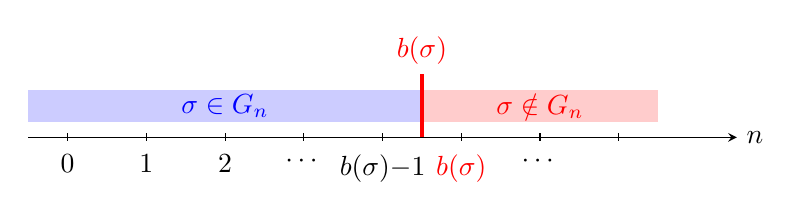
\begin{tikzpicture}[>=stealth]
  \draw[->] (0,0) -- (9,0) node[right] {$n$};
  \foreach \i in {0,...,7} \draw (\i+0.5,0.05) -- (\i+0.5,-0.05);
  \node[below] at (0.5,-0.1) {$0$};
  \node[below] at (1.5,-0.1) {$1$};
  \node[below] at (2.5,-0.1) {$2$};
  \node[below] at (3.5,-0.1) {$\cdots$};
  \node[below] at (4.5,-0.1) {$b(\sigma){-}1$};
  \node[below,red] at (5.5,-0.1) {$b(\sigma)$};
  \node[below] at (6.5,-0.1) {$\cdots$};
  % Fill indicator
  \fill[blue!20] (0,0.2) rectangle (5,0.6);
  \fill[red!20] (5,0.2) rectangle (8,0.6);
  \node[blue] at (2.5,0.4) {$\sigma \in G_n$};
  \node[red] at (6.5,0.4) {$\sigma \notin G_n$};
  \draw[very thick,red] (5,0) -- (5,0.8);
  \node[above,red] at (5,0.8) {$b(\sigma)$};
\end{tikzpicture}
\caption{分岐指標 $b(\sigma)$。$n < b(\sigma)$ では $\sigma \in G_n$，
$n \geq b(\sigma)$ では $\sigma \notin G_n$（分離条件のもとで）。}
\label{fig:ramification-break}
\end{figure}

\begin{remark}
将来の NT2 では\textbf{Hasse-Arf 定理}を扱う予定である：
上付番号の付け替え写像
$\varphi(t) = \int_0^t [G_0 : G_s]^{-1}\,ds$
を $\textsc{StructureTower}$ の \texttt{reindex} 操作として定式化し，
分岐ジャンプが整数値をとることを示す。
\end{remark}

% =============================================================================
\section{§NT1-5. idealPowTower への橋}
% =============================================================================

\subsection{二重フィルトレーション}

本節では，環と群の2つのフィルトレーションが同じ数論的現象を
異なる視点から記述することを形式化する。

\begin{figure}[H]
\centering
\begin{tikzcd}[row sep=2.5cm, column sep=3.5cm]
  \textsc{StructureTower}\,\mathbb{N}^{\mathrm{op}}\,R
  & \textsc{StructureTower}\,\mathbb{N}^{\mathrm{op}}\,G
  \\
  \texttt{idealPowTower}\,I
    \arrow[u, equal]
    \arrow[ur, dashed, "{\text{Artin 写像（NT3）}}" description]
  & \texttt{ramificationTower}\,\mathrm{rd}
    \arrow[u, equal]
    \arrow[ul, dashed, "{\text{作用の保存}}" description]
\end{tikzcd}
\caption{二重フィルトレーション。同じ添字集合 $\mathbb{N}^{\mathrm{op}}$ を共有する
環の塔と群の塔が，「ガロア対応」を通じて結ばれる。}
\label{fig:double-filtration}
\end{figure}

\subsection{塔保存作用}

\begin{definition}[塔保存作用]\label{def:tower-preserving-action}
  可換環 $R$，イデアル $I$，群 $G$ の $R$ への環準同型による作用
  $\mathrm{action}\colon G \to (R \xrightarrow{+*} R)$ が
  \textbf{塔保存的}（\texttt{TowerPreservingAction}）であるとは，
  \[
    \forall \sigma \in G,\;\forall n \in \mathbb{N},\;\forall x \in I^n\colon
    \quad \mathrm{action}(\sigma)(x) \in I^n
  \]
  が成立することをいう。
\end{definition}

\begin{theorem}[作用から塔射を構成]\label{thm:action-to-tower-hom}
  塔保存的作用に対し，各 $\sigma \in G$ に対する写像
  $x \mapsto \mathrm{action}(\sigma)(x)$
  は $\textsc{StructureTower}$ の射
  \[
    \texttt{actionToTowerHom}(\sigma)
    \;\in\;
    \Hom(\texttt{idealPowTower}\,I,\;\texttt{idealPowTower}\,I)
  \]
  を定める。
\end{theorem}

\begin{proof}
  \texttt{Hom} の \texttt{preserves} 条件：各 $n \in \mathbb{N}^{\mathrm{op}}$ と
  $x \in \mathrm{level}(n) = \lvert I^{\mathrm{ofDual}(n)}\rvert$ に対し，
  $\mathrm{action}(\sigma)(x) \in I^{\mathrm{ofDual}(n)} = \mathrm{level}(n)$
  が塔保存性から従う。
\end{proof}

\subsection{環から群への分岐部分群の誘導}

\begin{definition}[分岐部分集合]\label{def:ramification-subgroup}
  可換環 $R$，イデアル $I$，群 $G$ の作用 $\mathrm{action}$ に対し，
  \[
    \mathrm{ramificationSubgroup}(I,\mathrm{action},n)
    \;:=\;
    \bigl\{\,\sigma \in G \mid \forall x \in R,\;\mathrm{action}(\sigma)(x) - x \in I^n\,\bigr\}
  \]
  これは $G_n = \{\sigma \mid v(\sigma(x)-x) \geq n+1\}$ の抽象化である。
\end{definition}

\begin{theorem}[分岐部分集合の反単調性]\label{thm:ramification-antitone}
  $n \leq m \Rightarrow
  \mathrm{ramificationSubgroup}(I,\mathrm{action},m)
  \subseteq
  \mathrm{ramificationSubgroup}(I,\mathrm{action},n)$
\end{theorem}

\begin{proof}
  $I^m \subseteq I^n$（$m \geq n$ のとき $I^m \leq I^n$，
  \texttt{Ideal.pow\_le\_pow\_right}）から直接従う。
\end{proof}

\begin{figure}[H]
\centering
\begin{tikzcd}[row sep=2cm, column sep=1cm]
  R \supseteq I \supseteq I^2 \supseteq \cdots
    \arrow[d, leftrightarrow,
      "{\sigma \in G_n \;\Leftrightarrow\; \forall x \in R,\;\sigma(x)-x \in I^n}"
      description] \\
  G \supseteq G_0 \supseteq G_1 \supseteq \cdots
\end{tikzcd}
\caption{分岐部分集合の定義~\ref{def:ramification-subgroup} が，
環の塔と群の塔を結ぶ「橋」を与える。
$\sigma \in G_n \Leftrightarrow$ 「$\sigma$ は $I^n$ の精度で恒等写像に近い」。}
\label{fig:bridge}
\end{figure}

% =============================================================================
\section{全体のまとめと展望}
% =============================================================================

\subsection{NT1 で構築したこと}

\begin{enumerate}[label=\S NT1-\arabic*.]
  \item \textbf{部分群フィルトレーション塔}:
    反単調な部分群列 $f$ から $\texttt{subgroupFiltrationTower}(f)
    \in \textsc{StructureTower}\,\mathbb{N}^{\mathrm{op}}\,G$ を構成。
    各レベルでの単位元・逆元・乗法の閉性を確認。

  \item \textbf{正規鎖と閉包性}:
    $\texttt{subgroupFiltrationClosedTower}$:
    $\texttt{ClosedTower}\;\sgcl\;\mathbb{N}^{\mathrm{op}}$ が自動成立。
    正規部分群列のとき \texttt{conjugationHom}: 共役が塔の自己射を誘導。

  \item \textbf{分岐塔の公理的定義}:
    \texttt{RamificationData}: 反単調 + 正規 + 全体群条件。
    \texttt{HasCommutatorBound}: $[G_i,G_j] \leq G_{i+j}$
    — \texttt{idealPow\_mul\_mem} の群側対応物。

  \item \textbf{分離条件と脱出}:
    \texttt{IsSeparatedFiltration}: $\bigcap_n f(n) = \bot$（L5 の並行）。
    脱出定理: $\sigma \neq 1 \Rightarrow \exists n,\;\sigma \notin G_n$。
    \texttt{ramificationBreak}: 分岐指標 $b(\sigma) = \min\{n \mid \sigma \notin G_n\}$。

  \item \textbf{idealPowTower への橋}:
    \texttt{TowerPreservingAction}: 群作用が塔を保存する条件。
    \texttt{actionToTowerHom}: $\sigma \mapsto$ (idealPowTower の自己射)。
    \texttt{ramificationSubgroup}: 環のイデアル冪から群の分岐部分群を誘導。
\end{enumerate}

\subsection{NT2 以降の展望}

\begin{description}
  \item[NT2: Hasse-Arf 定理と reindex]
    分岐フィルトレーションの「上付番号」への変換：
    $\varphi(t) = \int_0^t [G_0 : G_s]^{-1}\,ds$
    を $\textsc{StructureTower}$ の \texttt{reindex} 操作として定式化。
    Hasse-Arf 定理：上付番号の分岐ジャンプは整数値
    $\Leftrightarrow$ \texttt{reindex} 後の塔が「整数格子上に集中する」。

  \item[NT3: 局所類体論と Tower Comparison]
    Artin 写像 $G^{\mathrm{ab}} \cong K^\times / N_{L/K}(L^\times)$
    を通じて，環側の塔（イデアル冪）と群側の塔（分岐群）を結ぶ。
    2つの $\textsc{StructureTower}$ 間の射として定式化。

  \item[NT4: 遠アーベル幾何への接続]
    副有限群のフィルトレーション
    $\pi_1(X)$ の開正規部分群列 $\to$ $\textsc{StructureTower}$。
    望月新一の Hodge 劇場：複数の塔の「リンク」の形式化。
\end{description}

\vspace{2em}
\begin{center}
\begin{tikzpicture}
  \node[draw,rounded corners,fill=blue!10,text width=6cm,align=center] (nt1)
    {\textbf{NT1}\\分岐塔の構成\\（本稿）};
  \node[draw,rounded corners,fill=green!10,text width=5cm,align=center,
    right=1.5cm of nt1] (nt2)
    {\textbf{NT2}\\Hasse-Arf + reindex};
  \node[draw,rounded corners,fill=orange!10,text width=5cm,align=center,
    right=1.5cm of nt2] (nt3)
    {\textbf{NT3}\\局所類体論\\Tower Comparison};
  \draw[->] (nt1) -- (nt2);
  \draw[->] (nt2) -- (nt3);
  \node[draw,rounded corners,fill=purple!10,text width=4cm,align=center,
    below=1.2cm of nt2] (nt4)
    {\textbf{NT4}\\遠アーベル幾何};
  \draw[->,dashed] (nt3) -- (nt4);
\end{tikzpicture}
\end{center}

% =============================================================================
\end{document}
